\documentclass[compress]{beamer}
\usepackage{ifthen,verbatim}

\title{Dimuon resolution in \\ $Z'$/graviton resonance searches}
\author{Jim Pivarski, Alexei Safonov}
\institute{Texas A\&M University}
\date{13 March, 2008}

\newcommand{\isnote}{}
\xdefinecolor{lightyellow}{rgb}{1.,1.,0.25}
\xdefinecolor{darkblue}{rgb}{0.1,0.1,0.7}

%% Uncomment this to get annotations
%% \def\notes{\addtocounter{page}{-1}
%%            \renewcommand{\isnote}{*}
%% 	   \beamertemplateshadingbackground{lightyellow}{white}
%%            \begin{frame}
%%            \frametitle{Notes for the previous page (page \insertpagenumber)}
%%            \itemize}
%% \def\endnotes{\enditemize
%% 	      \end{frame}
%%               \beamertemplateshadingbackground{white}{white}
%%               \renewcommand{\isnote}{}}

%% Uncomment this to not get annotations
\def\notes{\comment}
\def\endnotes{\endcomment}

\setbeamertemplate{navigation symbols}{}
\setbeamertemplate{headline}{\mbox{ } \hfill
\begin{minipage}{5.5 cm}
\vspace{-0.75 cm} \small
\end{minipage} \hfill
\begin{minipage}{4.5 cm}
\vspace{-0.75 cm} \small
\begin{flushright}
\ifthenelse{\equal{\insertpagenumber}{1}}{}{Jim Pivarski \hspace{0.2 cm} \insertpagenumber\isnote/\pageref{numpages}}
\end{flushright}
\end{minipage}\mbox{\hspace{0.2 cm}}\includegraphics[height=1 cm]{../cmslogo} \hspace{0.1 cm} \includegraphics[height=1 cm]{../tamulogo} \hspace{0.01 cm} \vspace{-1.05 cm}}

\begin{document}
\frame{\titlepage}

%% \begin{notes}
%% \item This is the annotated version of my talk.
%% \item If you want the version that I am presenting, download the one
%% labeled ``slides'' on Indico (or just ignore these yellow pages).
%% \item The annotated version is provided for extra detail and a written
%% record of comments that I intend to make orally.
%% \item Yellow notes refer to the content on the {\it previous} page.
%% \item All other slides are identical for the two versions.
%% \end{notes}

\begin{frame}
\frametitle{Dilepton resonances $>$ 1~TeV}

\textcolor{darkblue}{Generic signature and clean signal, especially for muons}

\mbox{ } \hfill \textcolor{darkblue}{$\Rightarrow$ potential for early discovery} \hfill \mbox{ }

\vfill
{\small Spin-1 $Z'$ models (my list) \hfill (benchmarks)}

\vspace{0.25 cm}
\begin{minipage}{\linewidth}\scriptsize
\begin{itemize}
\item Ad-hoc extension of the Standard Model \hfill $Z'_{SSM}$ \hspace{0.3 cm} \mbox{ }
\item Extra dimensions: heavy photon
\item $E(6)$ and $SO(10)$ GUTs {\it A.\ Leike, Phys.\ Rep.\ 317 (1999) 143.} \hfill $Z'_\psi$ \hspace{0.4 cm} \mbox{ }
\item Left-right symmetric models
\item String theory-inspired models {\it M.\ Cvetic and P.Langacker, 

Mod.\ Phys.\ Lett.\ A 11 (1996) 1247.}
\item Technicolor {\it C.T.\ Hill and E.H.\ Simmons Phys.\ Rep.\ 381 (2003) 235.}
\item The Little Higgs model {\it T.\ Han et al.\ Phys.\ Rev.\ D 67 (2003) 095004.}
\item Related to dark matter {\it K.\ Hsieh, R.N.\ Mohapatra, S.\ Nasri

Phys.\ Rev.\ D74 (2006)}
\item $Z'$-mediated SUSY breaking {\it P.\ Langacker, G.\ Paz, L.\ Wang, I.\ Yavin

Phys.\ Rev.\ Lett.\ 100, 041802 (2008)}
\end{itemize}
\end{minipage}

\vfill {\small Spin-2 graviton}

\vspace{0.25 cm}
\begin{minipage}{\linewidth}\scriptsize
\begin{itemize}
\item Randall-Sundrum extra dimensions {\it H.\ Davoudiasl, J.L.\ Hewett,} \hfill $G^*$ \hspace{0.4 cm} \mbox{ }

{\it T.G.\ Rizzo, Phys.Rev.Lett.\ 84 (2000)}
\end{itemize}
\end{minipage}
\end{frame}

\begin{frame}
\frametitle{Benchmarks at 100~pb$^{-1}$}

\begin{center}
\textcolor{darkblue}{$Z'_{SSM}$} \hspace{4 cm} \textcolor{darkblue}{$Z'_\psi$}

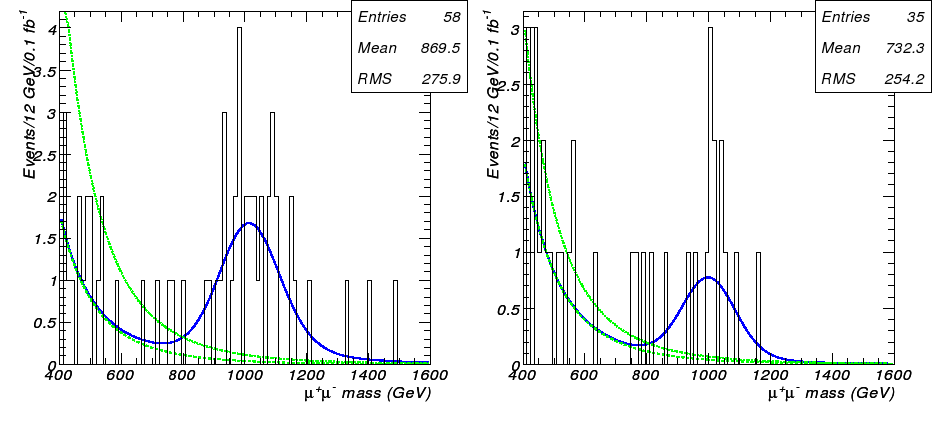
\includegraphics[width=\linewidth]{zprime_mc_experiments.png}

\begin{itemize}
\item Though the $Z'_{SSM}$ is 5 times wider than the $Z'_\psi$,
experimental widths are the same, primarily due to misalignment.
\item 100~pb$^{-1}$ misalignment scenario presented above
\end{itemize}

%% \vfill
%% 
\includegraphics[width=0.8\linewidth]{zprime_analysisnote_title.png}
\end{center}
\end{frame}

%% \begin{frame}
%% \begin{columns}
%% \column{0.6\linewidth}
%% 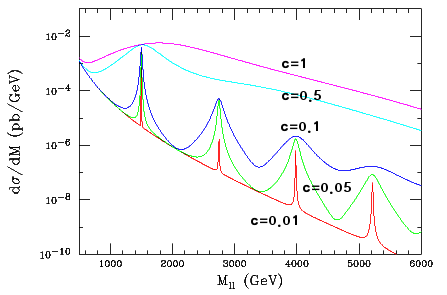
\includegraphics[width=\linewidth]{graviton_spectrum.png}

%% \column{0.4\linewidth}
%% \mbox{ }

%% \vspace{1 cm}
%% 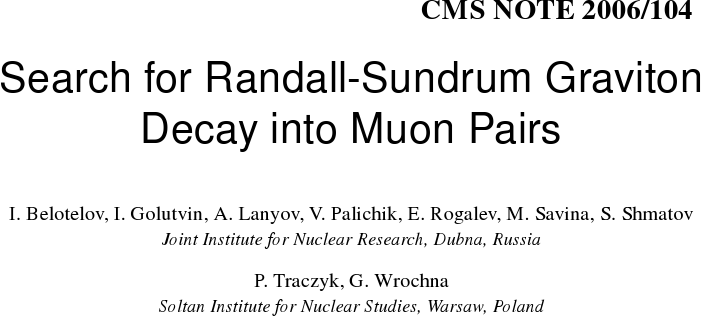
\includegraphics[width=\linewidth]{graviton_paper_title.png}
%% \end{columns}

%% \begin{center}
%% 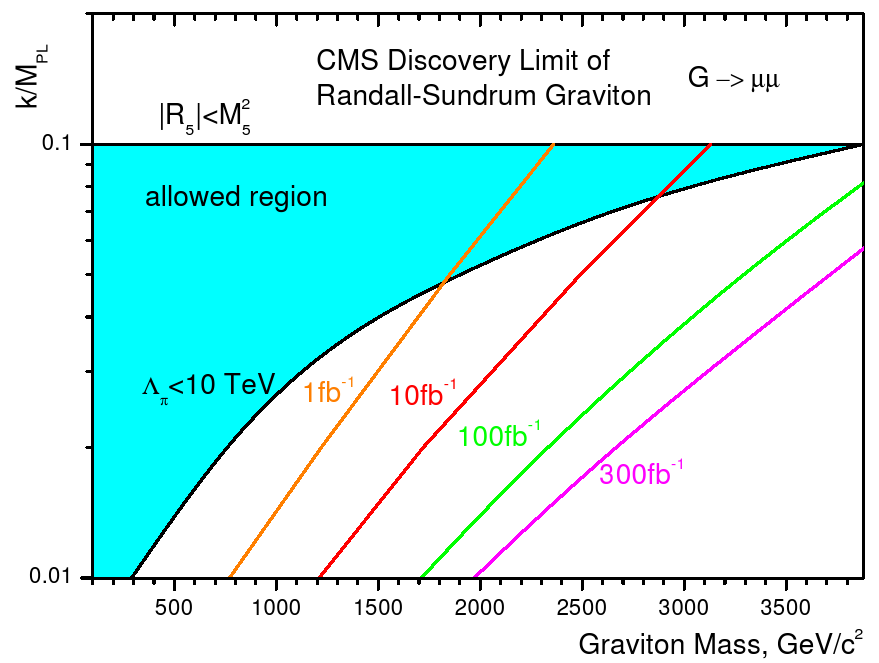
\includegraphics[width=0.6\linewidth]{graviton_reach.png}
%% \end{center}
%% \end{frame}

\begin{frame}
\frametitle{Steps toward discovery}
\mbox{\begin{minipage}{\linewidth}
\begin{itemize}
\item \textcolor{darkblue}{Understanding backgrounds:}
\begin{itemize}
\item relevant for discovery of a real TeV dimuon excess \\
\mbox{ } \hfill (broad/overlapping resonances, unparticles, PDFs at 14~TeV)
\end{itemize}
\end{itemize}
\end{minipage}}

\vspace{0.4 cm}
\textcolor{blue}{\fbox{\begin{minipage}{\linewidth}
\begin{itemize}
\item \textcolor{darkblue}{Resolution, momentum scale:}
\begin{itemize}
\item discovery of a resonance ($Z'$ or graviton)
\item measurement of its mass, upper limit on width
\end{itemize}
\end{itemize}
\end{minipage}}}

\vspace{0.4 cm}
\mbox{\begin{minipage}{\linewidth}
\begin{itemize}
\item \textcolor{darkblue}{Efficiency, PDF uncertainties:}
\begin{itemize}
\item measurement of its cross-section \\
\mbox{ } \hfill (weak discriminant between $Z'$ models)
\end{itemize}
\end{itemize}
\end{minipage}}

\vspace{0.4 cm}
\mbox{\begin{minipage}{\linewidth}
\begin{itemize}
\item \textcolor{darkblue}{Angular distributions:}
\begin{itemize}
\item measurement of its spin (determine $Z'$ versus graviton)
\item forward-backward asymmetry (determine $Z'$ model)
\end{itemize}
\end{itemize}
\end{minipage}}

\vspace{0.7 cm}
This talk will focus on dimuon resolution

%% \hspace{-0.83 cm} \textcolor{darkblue}{\Large Outline2}
\end{frame}

%% \begin{frame}
%% \frametitle{Cuts and backgrounds}

%% \vfill
%% \begin{itemize}
%% \item Isolation cut:
%% \begin{itemize}\setlength{\itemsep}{0.1 cm}
%% \item $\Sigma p_T$ $<$ 10~GeV in a cone $\Delta R = \sqrt{(\Delta \phi)^2 + (\Delta \eta)^2}$ $<$ 0.3 around each muon
%% \end{itemize}
%% \item Remainder is irreducible Drell-Yan (\textcolor{red}{red line} in plots below)
%% \item Let background term float in peak fit
%% \end{itemize}

%% \begin{center}
%% opposite sign \hspace{3 cm} same sign

%% 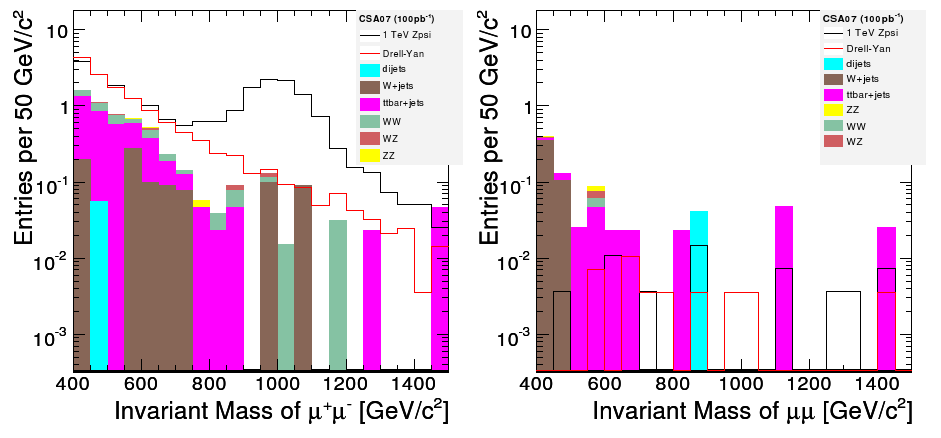
\includegraphics[width=\linewidth]{backgrounds.png}
%% \end{center}

%% \vspace{-0.5 cm}
%% \mbox{ } \hfill \it \small M.\ Chen (Beijing), Univ.\ of Florida
%% \end{frame}

\begin{frame}
\frametitle{Intrinsic resolution}
TeV muons shower in iron
\begin{center}
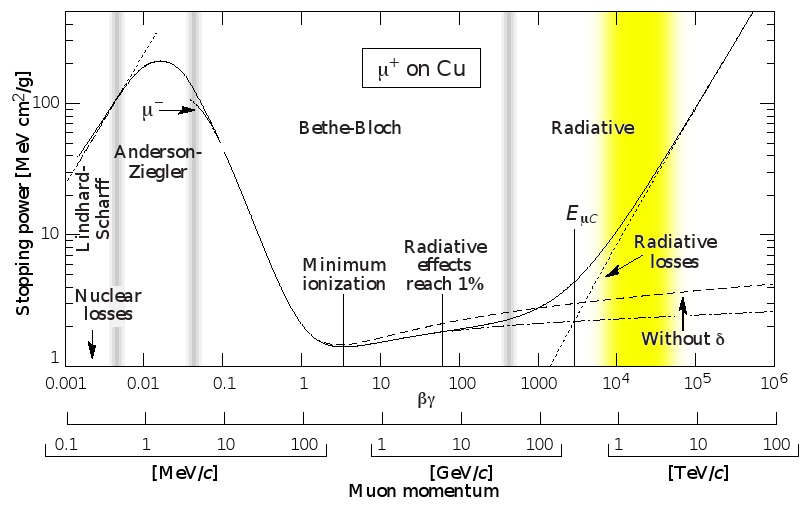
\includegraphics[width=0.7\linewidth]{pdgplot.png}
\end{center}

\begin{columns}
\column{0.5\linewidth}
\small
\begin{itemize}
\item Showers that start deep in the iron are suppressed
\item Some chambers flooded with extra hits, others are fine
\end{itemize}

\column{0.5\linewidth}
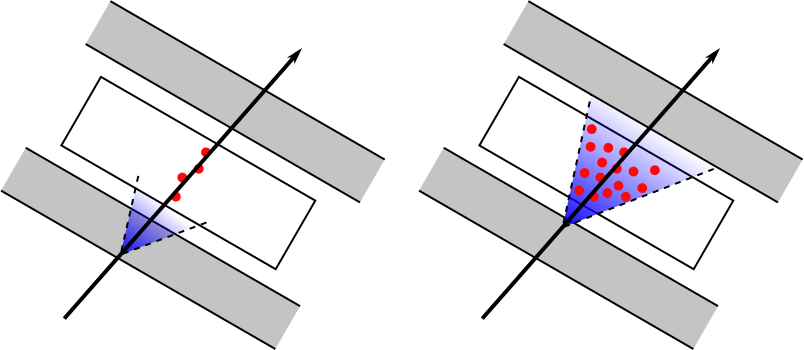
\includegraphics[width=\linewidth]{showering_hits.png}
\end{columns}
\end{frame}

\begin{frame}
\frametitle{Optimizing track fits}
\begin{columns}
\column{0.7\linewidth}
\small
\begin{enumerate}
\item Identify chambers with showers, apply tight cuts on hits (``Picky Muon Reconstruction'')
\item First muon station is most important for momentum resolution,
keep only first station (``Truncated Muon Reconstruction'')
\item Run both and select best \mbox{track $\chi^2$ (``Tune N, P'') \hspace{-1 cm}}
\end{enumerate}

\column{0.3\linewidth}
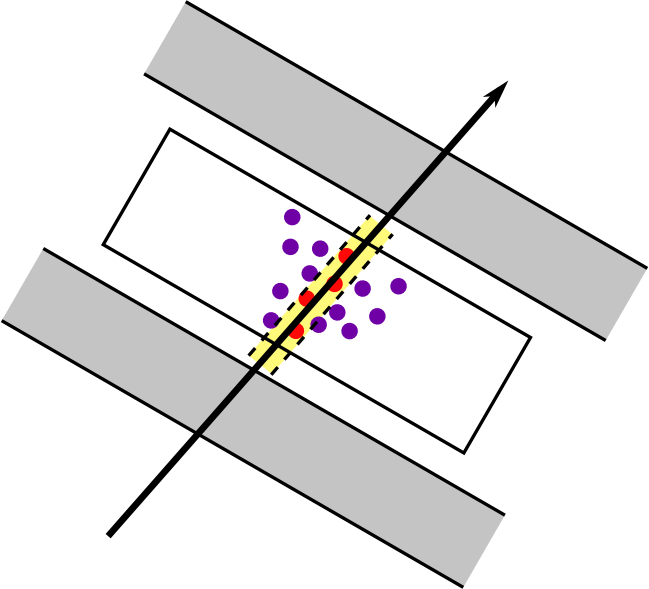
\includegraphics[width=\linewidth]{showering_hits2.png}
\end{columns}

\begin{center}
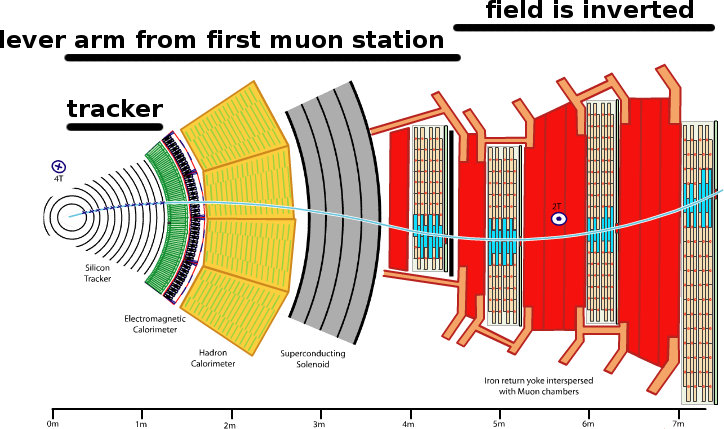
\includegraphics[width=0.7\linewidth]{muon_trajectory.png}
\end{center}
\end{frame}

\begin{frame}
\frametitle{Comparison of 6 algorithms}

\vfill
\begin{itemize}
\item Optimize for statistical significance of peak over backgrounds
\item All optimized variants are better than the default, but it's unclear which is best
\begin{itemize}
\item Might depend on misalignment (untested)
\item Might prefer wider central Gaussian to long tails
\end{itemize}
\end{itemize}

\scriptsize \mbox{ } \hfill \it Piotr Traczyk (Warsaw) 

\vspace{-0.38 cm}
\begin{center}
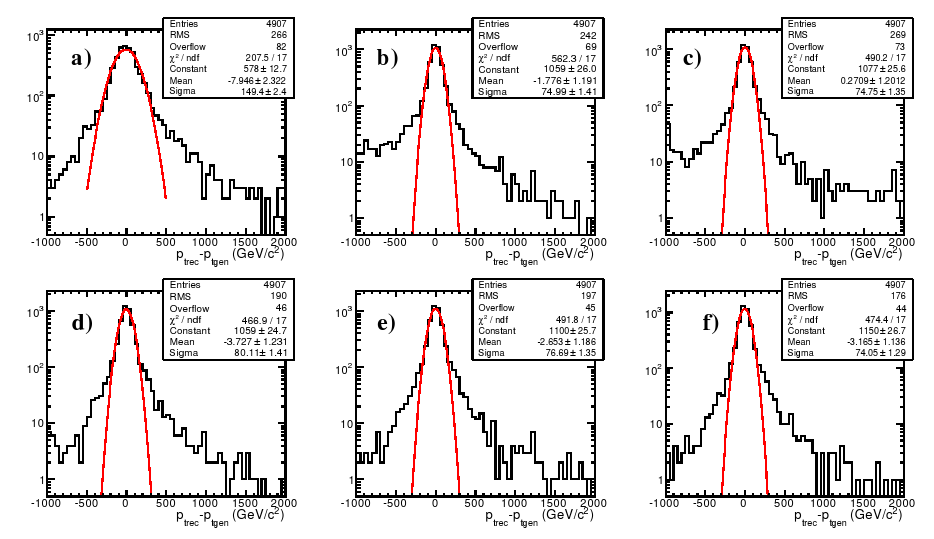
\includegraphics[width=0.8\linewidth]{compare_reconstructors.png}

\scriptsize (a) default (keep all hits), (b) truncated, (c) picky, (d-f) tuned cocktails
\end{center}
\end{frame}

\begin{frame}
\frametitle{Misalignment}

\vfill
\begin{itemize}
\item Three sources:
\begin{itemize}
\item Internal tracker misalignment
\item Internal muon system misalignment
\item Relative misalignment of tracker and muon system
\end{itemize}
\end{itemize}

Momentum resolution with and without tracker, muon system
\begin{itemize}
\item Tracker dominates below 1--2~TeV, but not above
\end{itemize}
\begin{center}
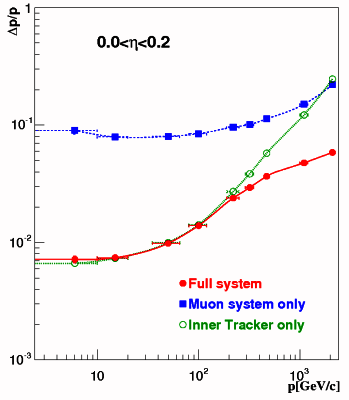
\includegraphics[width=0.4\linewidth]{Figure_001-005-a.png} 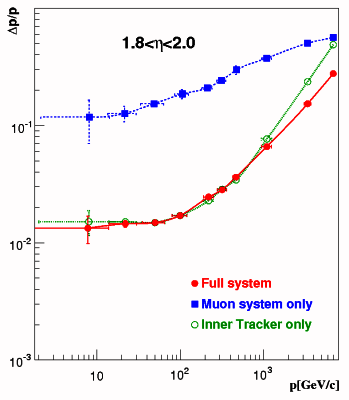
\includegraphics[width=0.4\linewidth]{Figure_001-005-b.png}
\end{center}
\end{frame}

\begin{frame}
\frametitle{100~pb$^{-1}$ misalignment scenario}

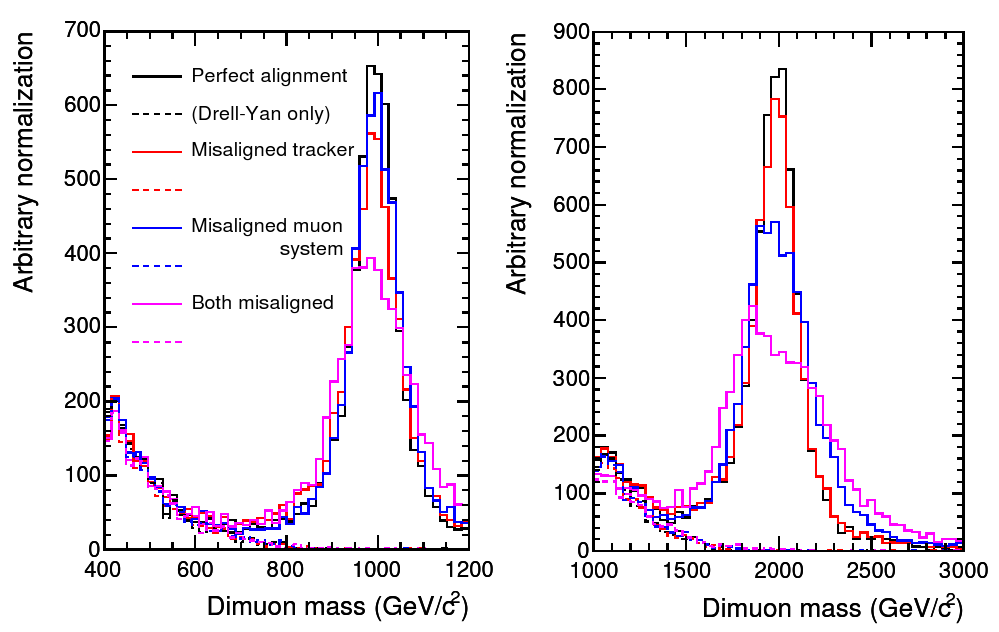
\includegraphics[width=\linewidth]{misaligned_spectra.png}

\begin{itemize}
\item \textcolor{blue}{Muon misalignment} matters a lot more at 2~TeV
\item Expected misalignment is not sufficient to smear a lot of Drell-Yan up in mass
\end{itemize}
\end{frame}

\begin{frame}
\frametitle{Alignment systems}

\textcolor{darkblue}{Tracker}
\begin{itemize}
\item Laser alignment system (LAS) provides first alignment
\item Track-based alignment: vary presumed sensor positions until track $\chi^2$ are minimized
\begin{itemize}
\item HIP algorithm: iteratively fit tracks and update sensor positions
\item MillePede and Kalman-based algorithms: fit tracks and sensor positions simultaneously
\end{itemize}
\item Non-IP tracks (cosmic rays, beam-halo) are crucial for breaking degeneracies along ``weak modes''
\end{itemize}

\textcolor{darkblue}{Muon system}
\begin{itemize}
\item Hardware alignment system: laser position monitors and analog calipers
\item Track-based alignment
\begin{itemize}
\item weight tracker hits more heavily to align muon chambers relative to the tracker
\item HIP and MillePede algorithms
\end{itemize}
\end{itemize}

%% \begin{center}
%% 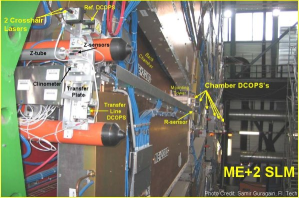
\includegraphics[height=3 cm]{hw_alignment2.png}
%% 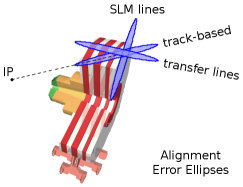
\includegraphics[height=3 cm]{error_ellipses.png}
%% \end{center}
\end{frame}

\begin{frame}
\frametitle{Muon misalignment scenarios}

\begin{itemize}
\item \textcolor{darkblue}{CSA07}
\begin{itemize}
\item \textcolor{darkblue}{10~pb$^{-1}$ scenario:} represents state with no track-based input
\item \textcolor{darkblue}{100~pb$^{-1}$ scenario:} some track-based input
\item Due to a mistake, the 100~pb$^{-1}$ scenario is {\it worse} than the 10~pb$^{-1}$ at high mass
\end{itemize}

\item \textcolor{darkblue}{Output of track-based alignment algorithm (HIP)}

\begin{itemize}
\item \textcolor{darkblue}{10~pb$^{-1}$ with and without 10~pb$^{-1}$ tracker misalignment}

\item \textcolor{darkblue}{100~pb$^{-1}$ with and without 100~pb$^{-1}$ tracker misalignment}

\item \textcolor{darkblue}{3 trials each:} to quantify dependence on initial condition

\item Doesn't incorporate improvements discovered since Nov.\ 2007

\item Tuned for 10~pb$^{-1}$; makes poor use of extra tracks in 100~pb$^{-1}$
\end{itemize}

\item \textcolor{darkblue}{CSA08}
\begin{itemize}
\item \textcolor{darkblue}{0~pb$^{-1}$ scenario:} represents state with no track-based input
\item \textcolor{darkblue}{10~pb$^{-1}$ scenario:} combination of hardware and track-based
\item \textcolor{darkblue}{100~pb$^{-1}$ scenario:} more heavily track-based, still doesn't scale

\mbox{ } \hfill as $\sqrt{10}$ relative to 10~pb$^{-1}$ scenario
\item Mistake fixed (and new scenarios are more detailed, precise)
\end{itemize}
\end{itemize}
\end{frame}

\begin{frame}
\frametitle{Muon track resolution}

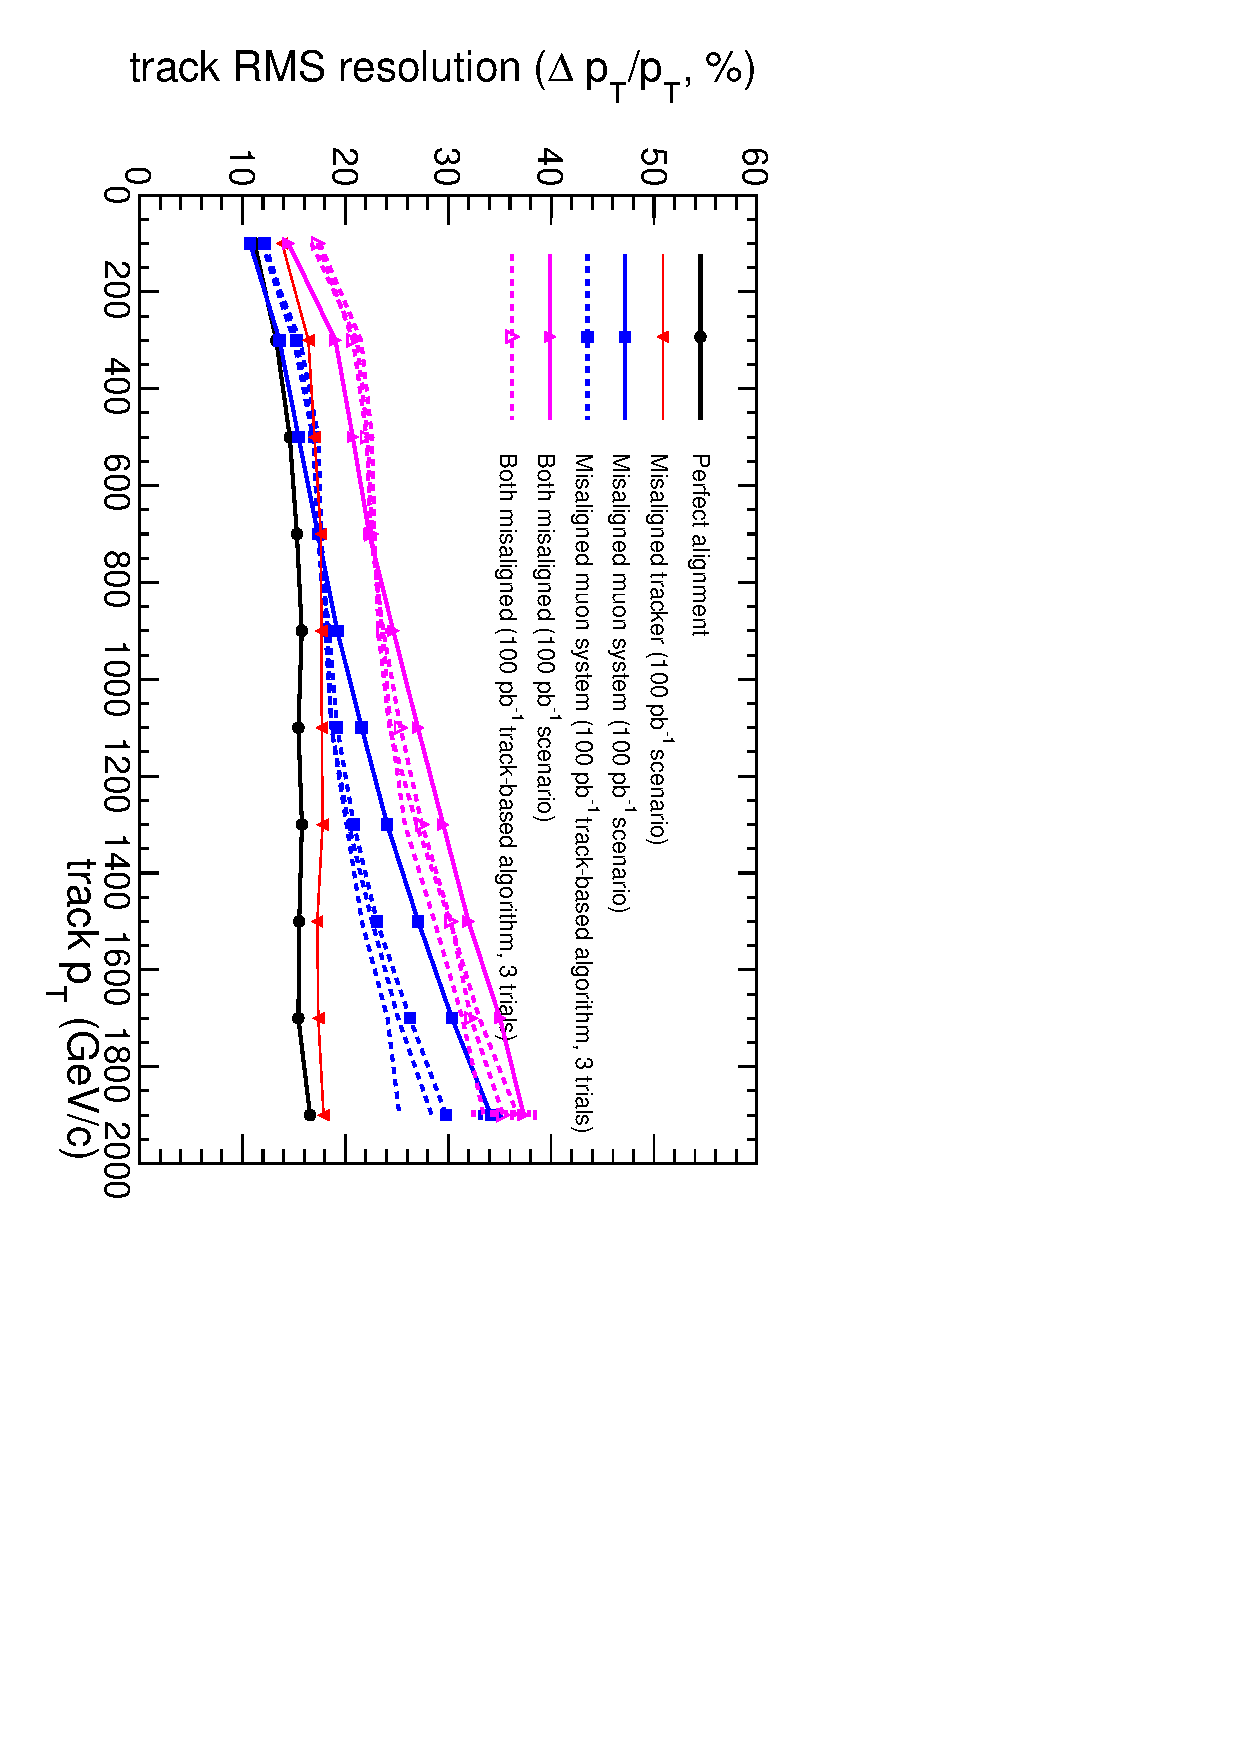
\includegraphics[height=\linewidth, angle=90]{ZSSM_Align_TrackRes_color-100.pdf}

\begin{itemize}
\item $p_T$ resolution is curvature resolution: $\displaystyle \bigg(\frac{\Delta {p_T}}{p_T}\bigg) = \bigg(\frac{\Delta \kappa}{\kappa}\bigg)$
\end{itemize}
\end{frame}

\begin{frame}
\frametitle{Dimuon mass resolution}

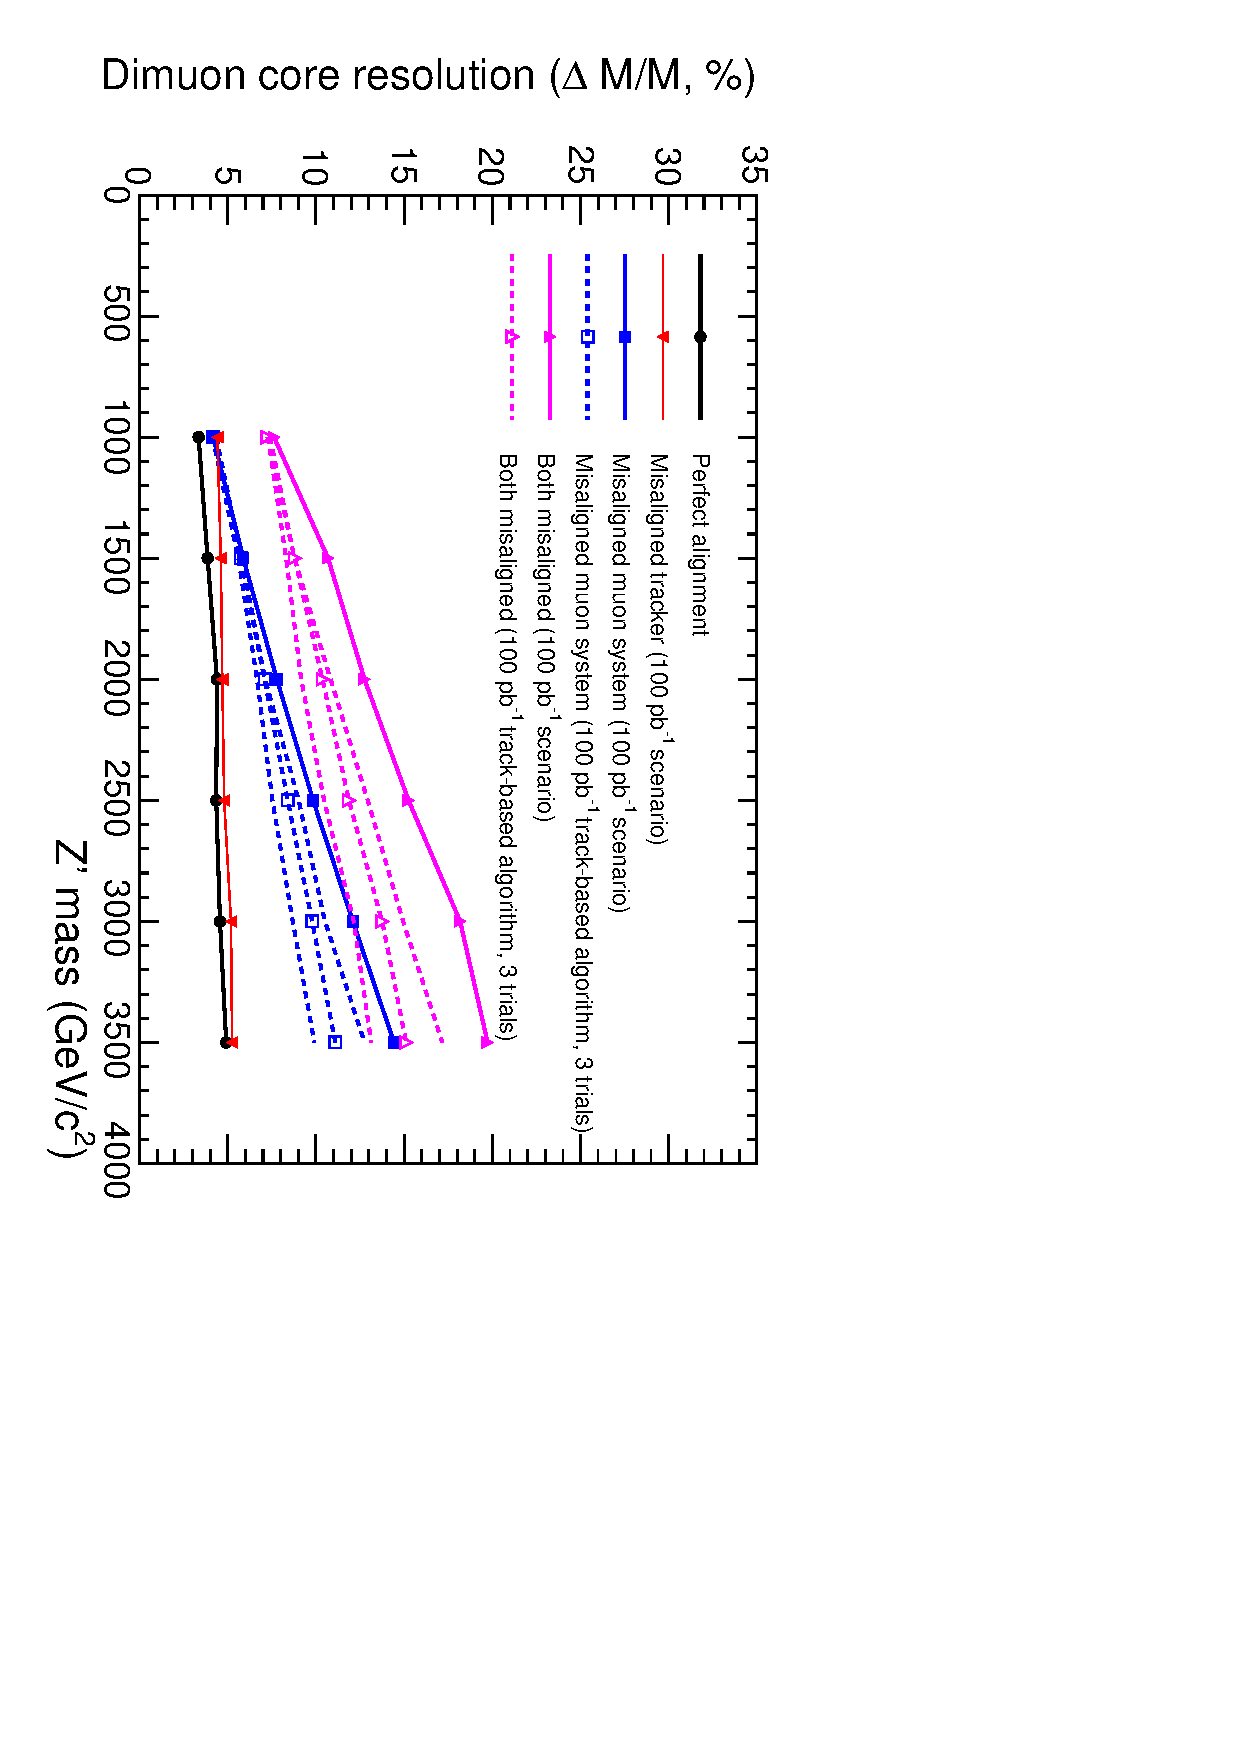
\includegraphics[height=\linewidth, angle=90]{ZSSM_Align_MassRes_color-100.pdf}

\begin{itemize}
\item ``Core resolution'' is $\sigma$ of the Gaussian fit, with the fit range restricted to $-1.5\sigma$ through $1.5\sigma$
\end{itemize}
\end{frame}

\begin{frame}
\frametitle{Dimuon mass resolution}

\begin{itemize}
\item Comparison of 10 and 100~pb$^{-1}$

\item Plot from {\small CMS AN 2007/038} (internal)
\end{itemize}

\vspace{-0.5 cm}
\begin{center}
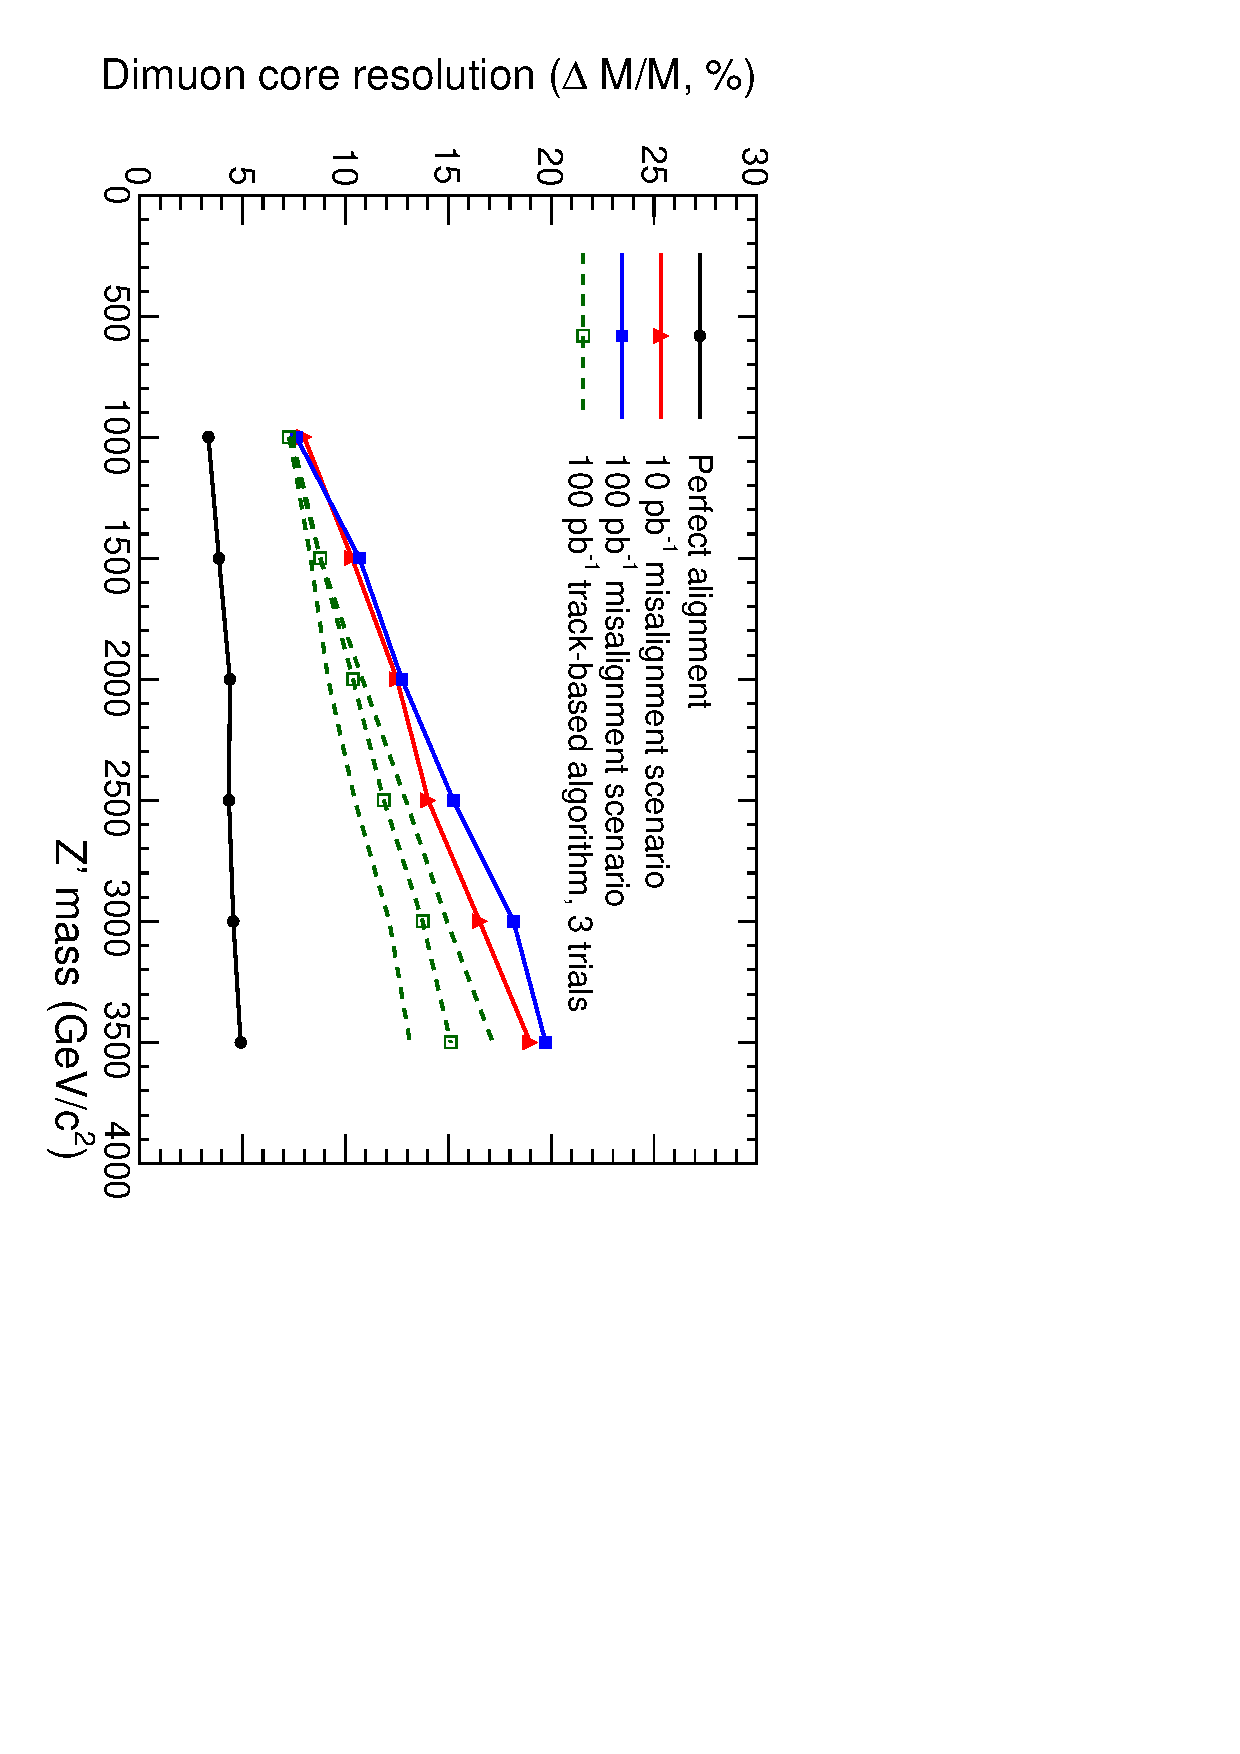
\includegraphics[height=0.9\linewidth, angle=90]{ZSSM_Align10-100_MassRes_color.pdf}
\end{center}

\vspace{-0.5 cm}
\begin{itemize}
\item Bottom line: track-based test confirms that misalignment
scenarios are in the right ballpark
\end{itemize}
\end{frame}

\begin{frame}
\frametitle{New CSA08 scenarios}

\vspace{0.5 cm}
Check that they scale appropriately with a 3.5~TeV $Z'$

\begin{center}
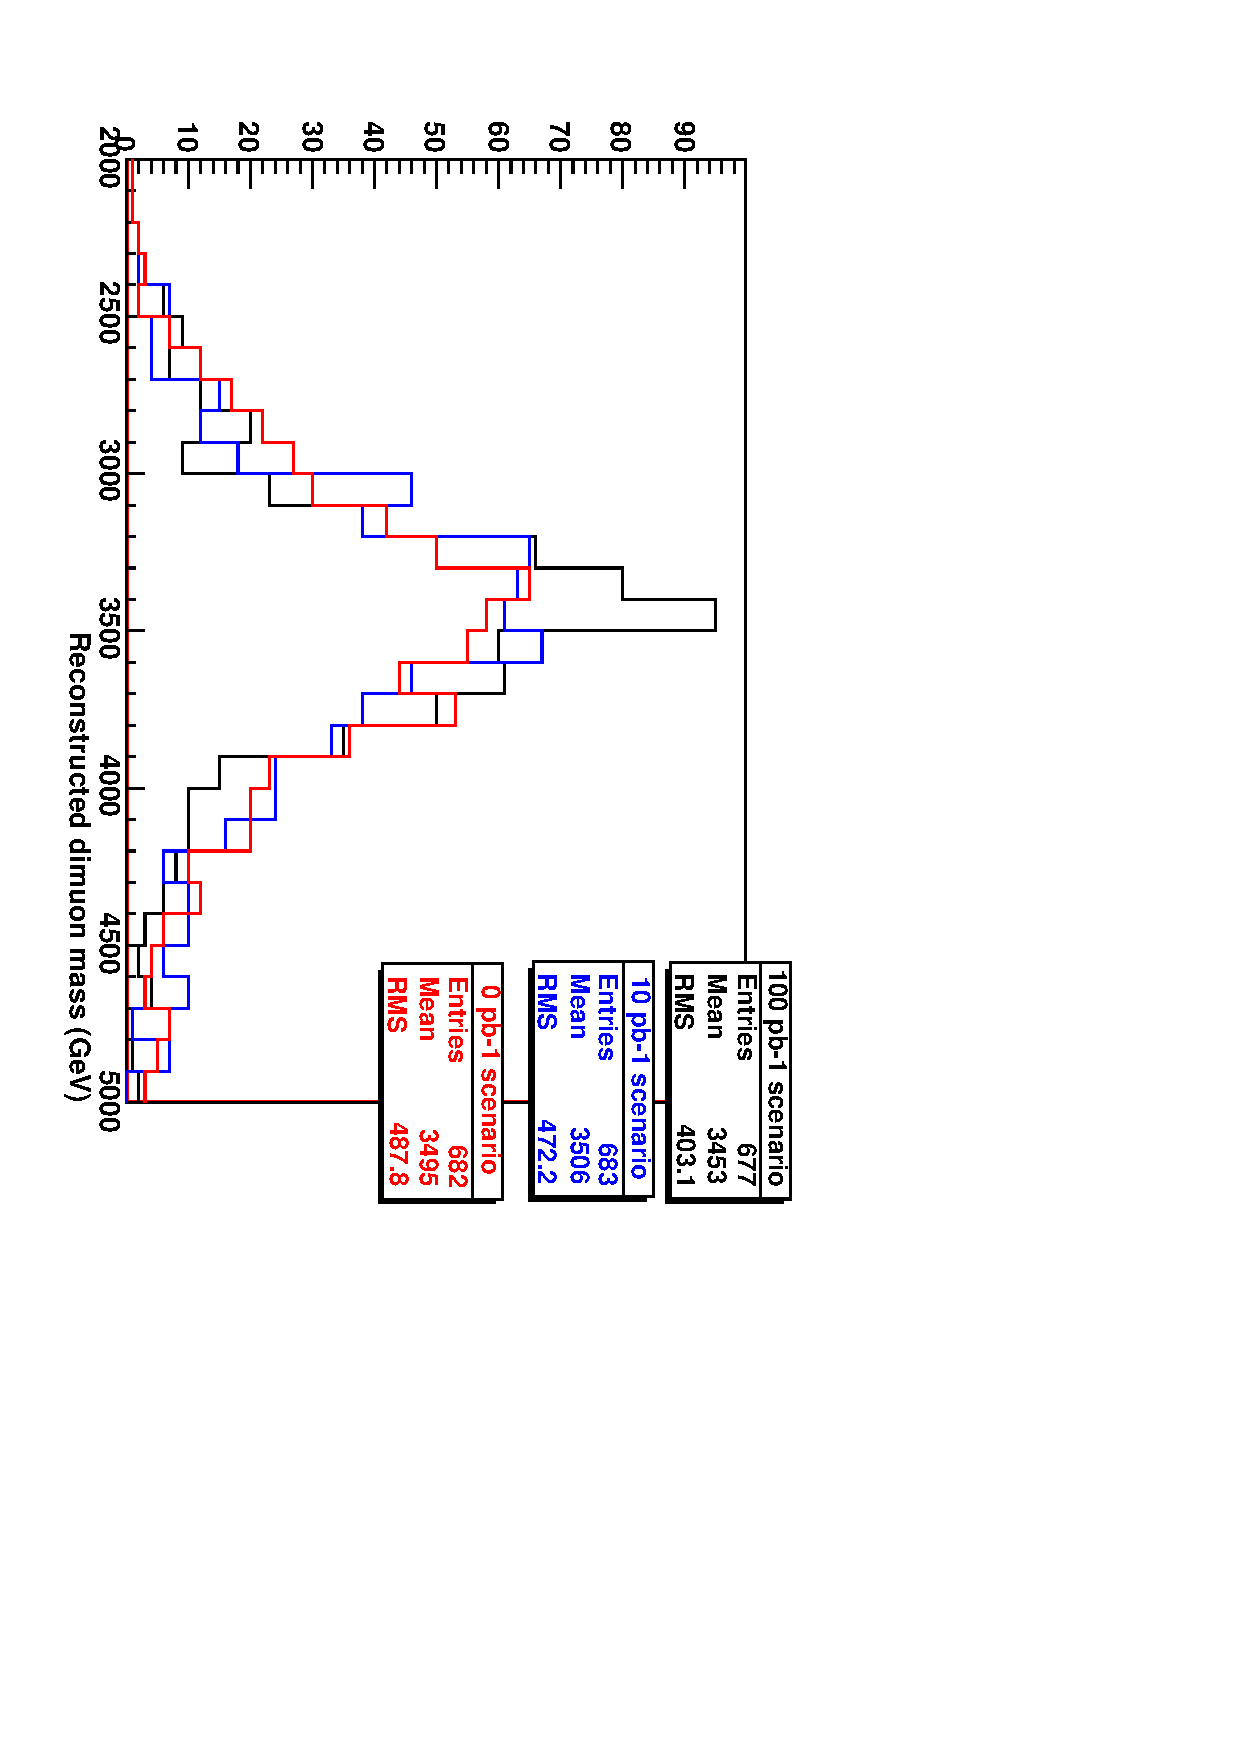
\includegraphics[height=0.8\linewidth, angle=90]{newscenarios_zprimetest.pdf}

\vspace{0.5 cm}
\begin{tabular}{c c c c}
ideal (not shown) & 100~pb$^{-1}$ & \textcolor{blue}{10~pb$^{-1}$} & \textcolor{red}{0~pb$^{-1}$} \\\hline
5\% & 11.5\% & \textcolor{blue}{13.5\%} & \textcolor{red}{13.9\%}
\end{tabular}

\end{center}
\end{frame}

\begin{frame}
\frametitle{Effect on energy scale}

\textcolor{darkblue}{``Bias'':} shift in mean of momentum/mass relative to generated

\vspace{-0.25 cm}
\begin{columns}
\column{0.5\linewidth}
\begin{center} Track momentum \end{center}

\vspace{-0.25 cm}
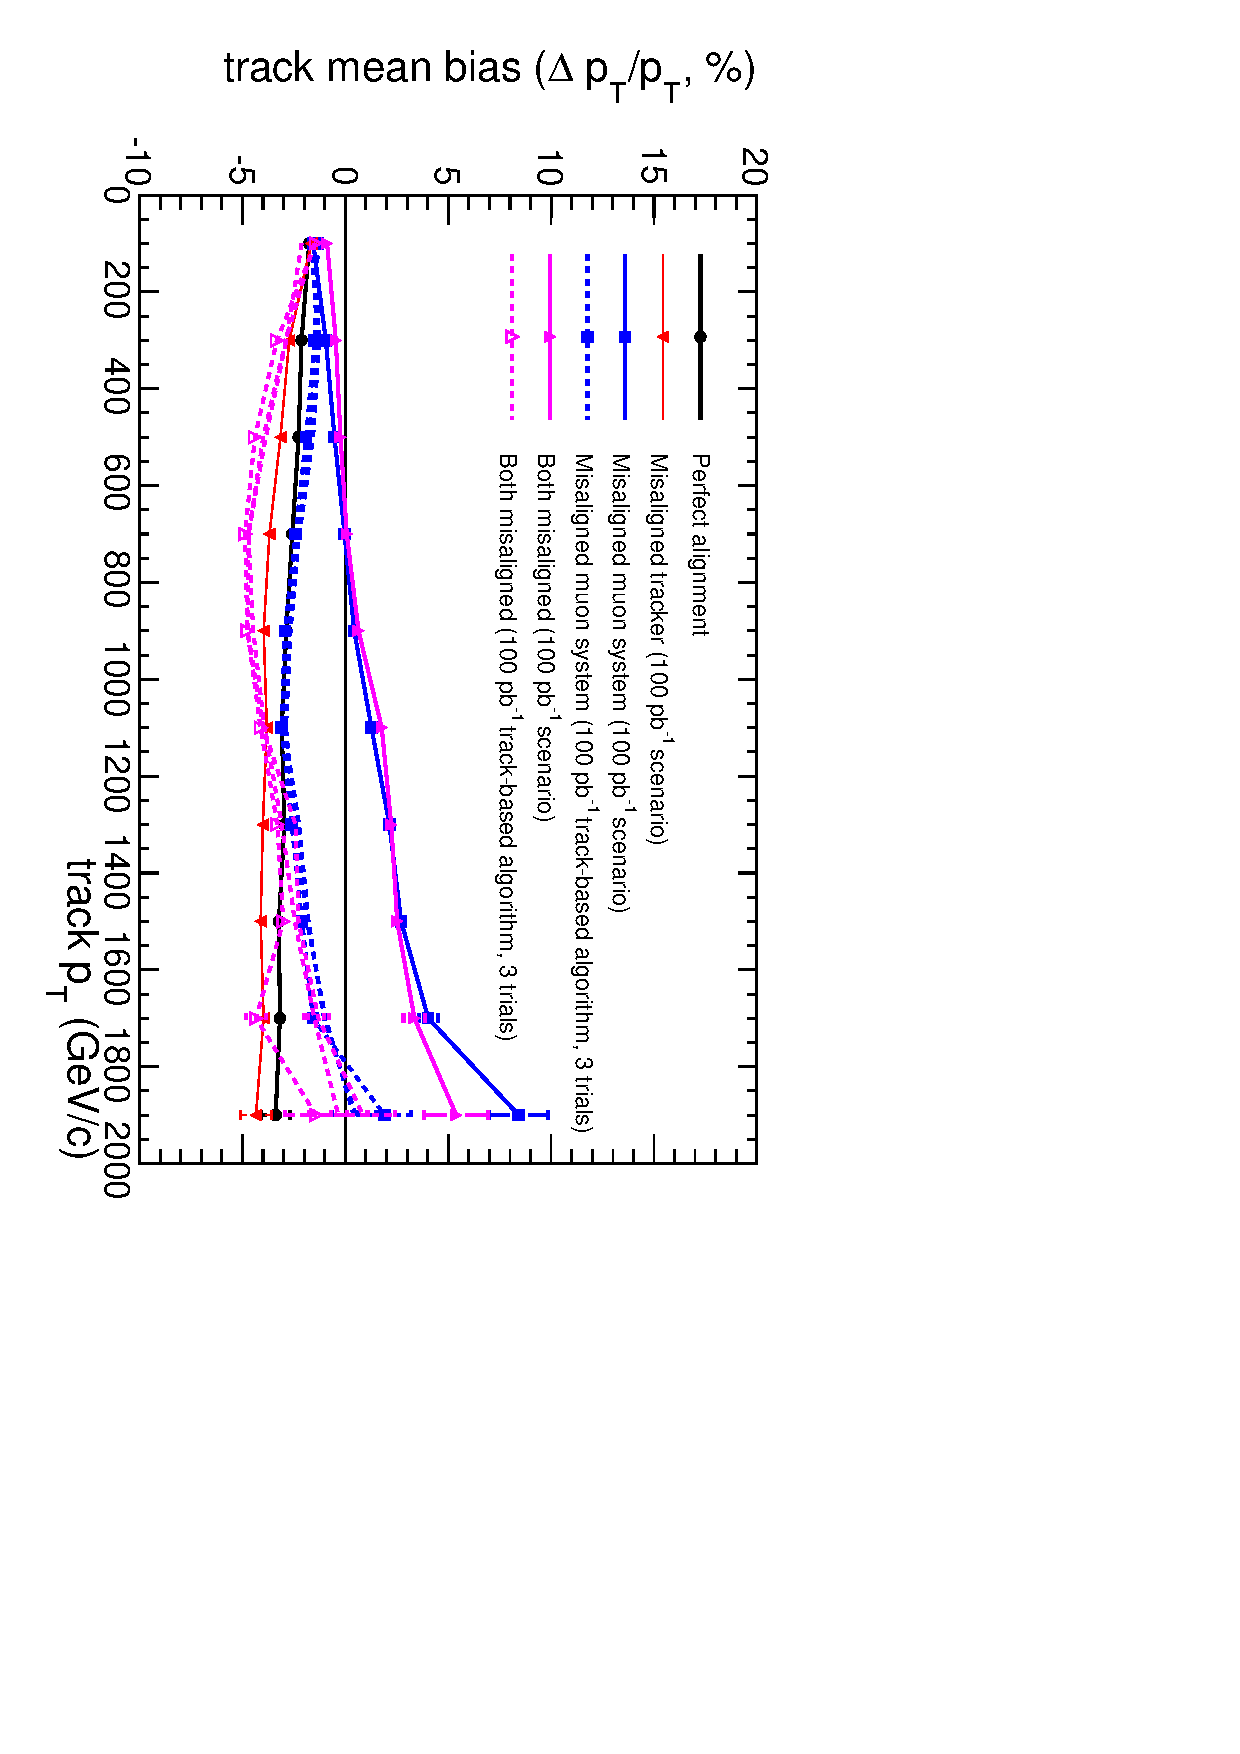
\includegraphics[height=1.1\linewidth, angle=90]{ZSSM_Align_TrackBias_color-100.pdf}
\column{0.5\linewidth}
\begin{center} Dimuon mass \end{center}

\vspace{-0.25 cm}
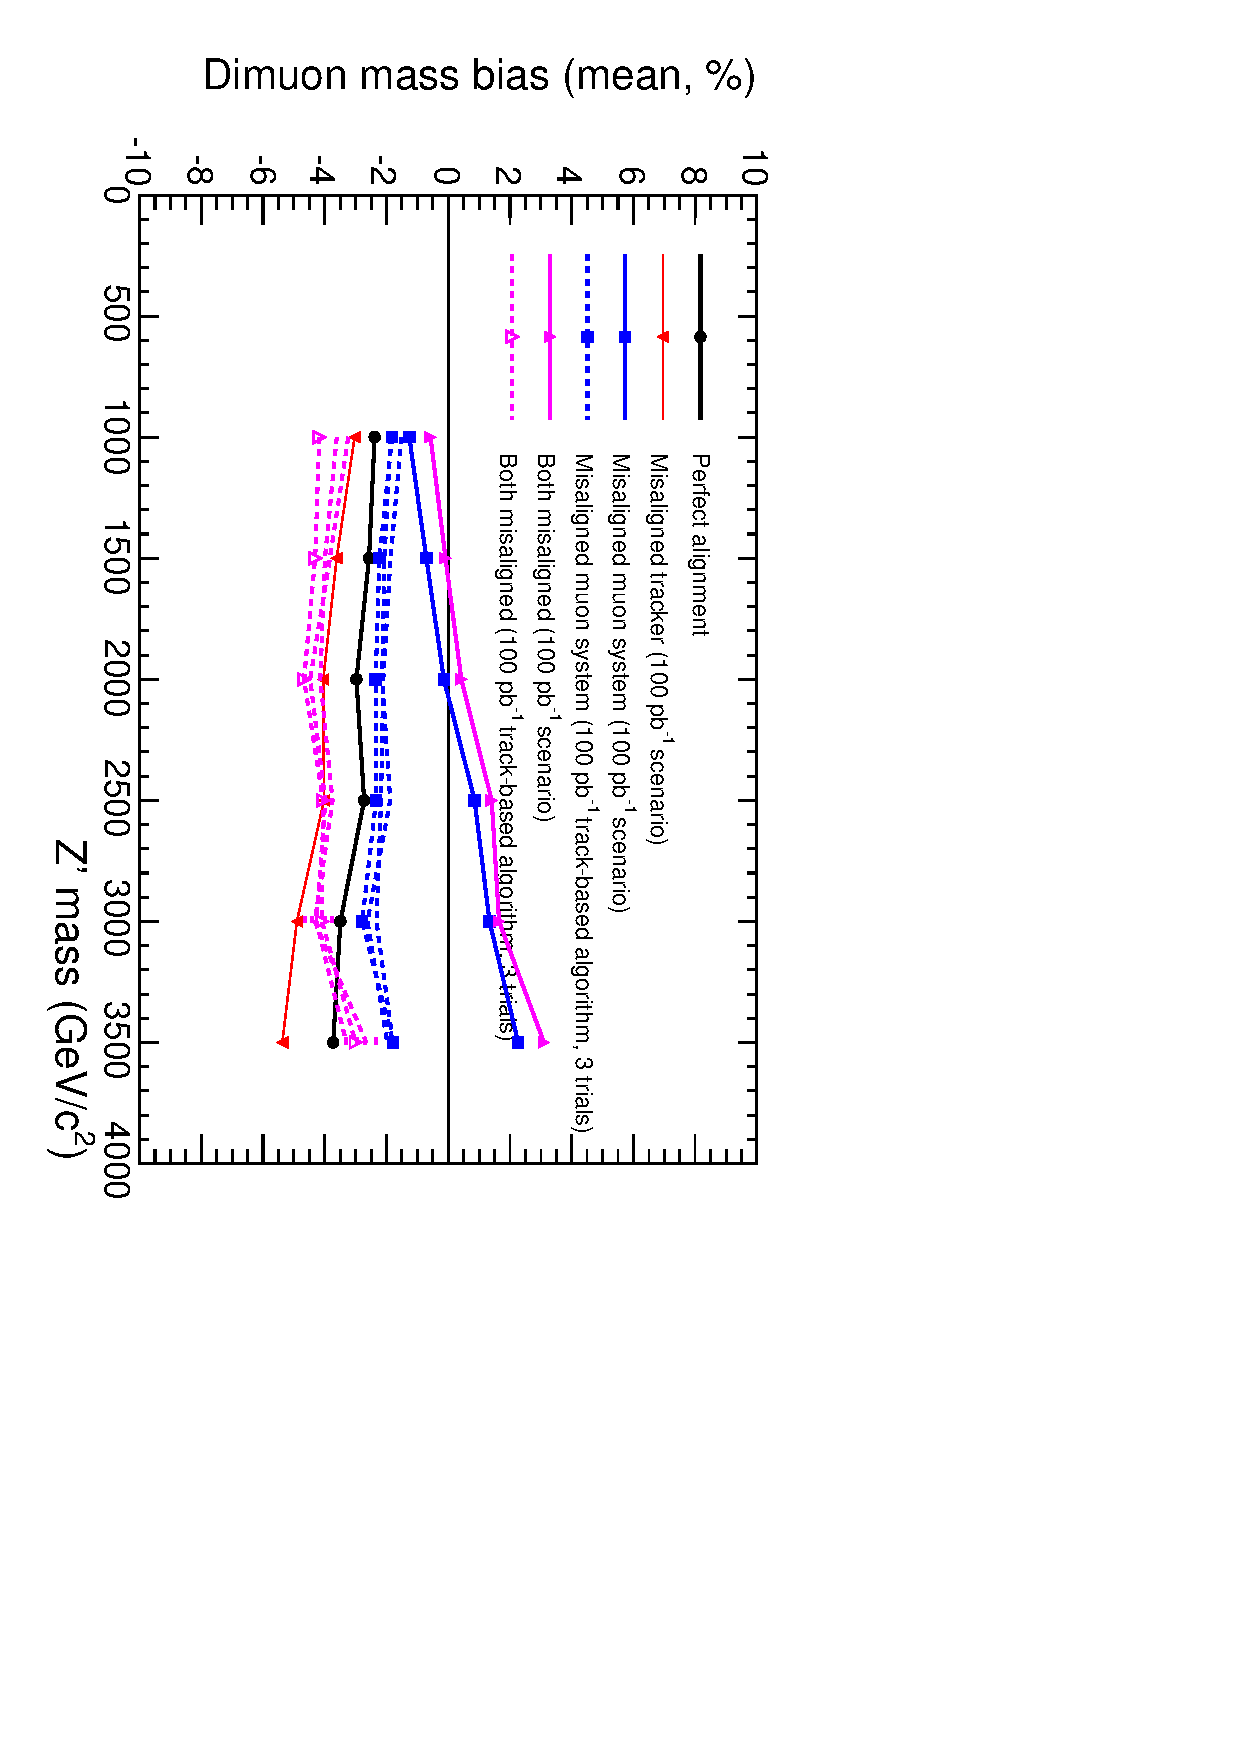
\includegraphics[height=1.1\linewidth, angle=90]{ZSSM_Align_MassBiasMean_color-100.pdf}
\end{columns}

\vspace{0.25 cm}
\begin{itemize}
\item Dimuon bias follows track momentum bias
\item Track-based results and ideal are both negative (about $-3$\%)
\item Misalignment scenarios are both positive
\item Nothing is more than 5\% ($\Delta/$total)
\end{itemize}
\end{frame}

\begin{frame}
\frametitle{Open projects in resolution}

\textcolor{darkblue}{Listed by Slava as ``no one working on it, as far as I know''}

\vspace{0.5 cm}
\begin{itemize}\setlength{\itemsep}{0.5 cm}
\item Determining resolution from data
\begin{itemize}\setlength{\itemsep}{0.25 cm}
\item Perhaps a bottom-up approach: measure residuals and
misalignments, then infer track resolution from MC?
\end{itemize}

\item TeV momentum scale
\begin{itemize}\setlength{\itemsep}{0.25 cm}
\item ``Bias'' described on previous slide is the first correction
\item Can this be determined from data?
\end{itemize}

\end{itemize}
\end{frame}

\begin{frame}
\frametitle{Conclusions}
\begin{itemize}\setlength{\itemsep}{0.35 cm}
\item TeV muon resolution is key for early physics

\item Intrinsic resolution $\sim$5\% due to muon showering

\begin{itemize}
\item Can be reduced to $\sim$2.5\% by dropping excess hits
\end{itemize}

\item Misaligned resolution $\sim$7.5 to 15\% \mbox{(1 to 3.5~TeV) \hspace{-1 cm}}

\begin{itemize}\setlength{\itemsep}{0.1 cm}
\item CSA07 scenarios and track-based output in rough agreement
\item Does not include known improvements
\end{itemize}

\item Mistake in the CSA07 scenarios led to 10~pb$^{-1}$ being better
than 100~pb$^{-1}$

\begin{itemize}\setlength{\itemsep}{0.1 cm}
\item Mistake has been corrected in CSA08
\item CSA08 scenarios include more information about distribution of
uncertainties, with guidance from track-based output
\end{itemize}

\item There are at least two open projects

\end{itemize}
\label{numpages}
\end{frame}

\section*{Backup slides}
\begin{frame}
\begin{center}
\Huge \textcolor{blue}{Backup slides}
\end{center}
\end{frame}

\begin{frame}
\frametitle{Effect on efficiency?}

\begin{itemize}
\item Misalignment has a negligible effect on trigger efficiency
\item and reconstruction efficiency:
\end{itemize}

\begin{center}
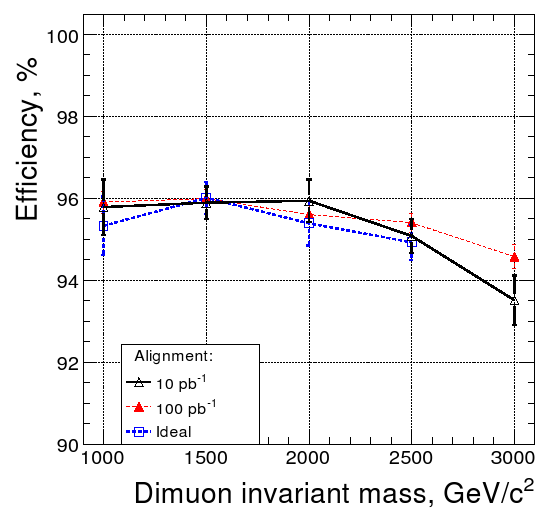
\includegraphics[width=0.6\linewidth]{reconstruction_efficiency.png}
\end{center}
\end{frame}

\end{document}
